Under vil vi presentere relevante funn og resultater relatert til problemstillingen. Data er hentet gjennom spørreundersøkelsen og dybdeintervjuene.

\indent \newline
Undersøkelsen er utarbeidet gjennom ledelsesteori presentert tidligere i oppgaven. Formålet er å vurdere dagens ledelse ved Involve. Resultatene er som følger:

\begin{figure}[H]
\centering
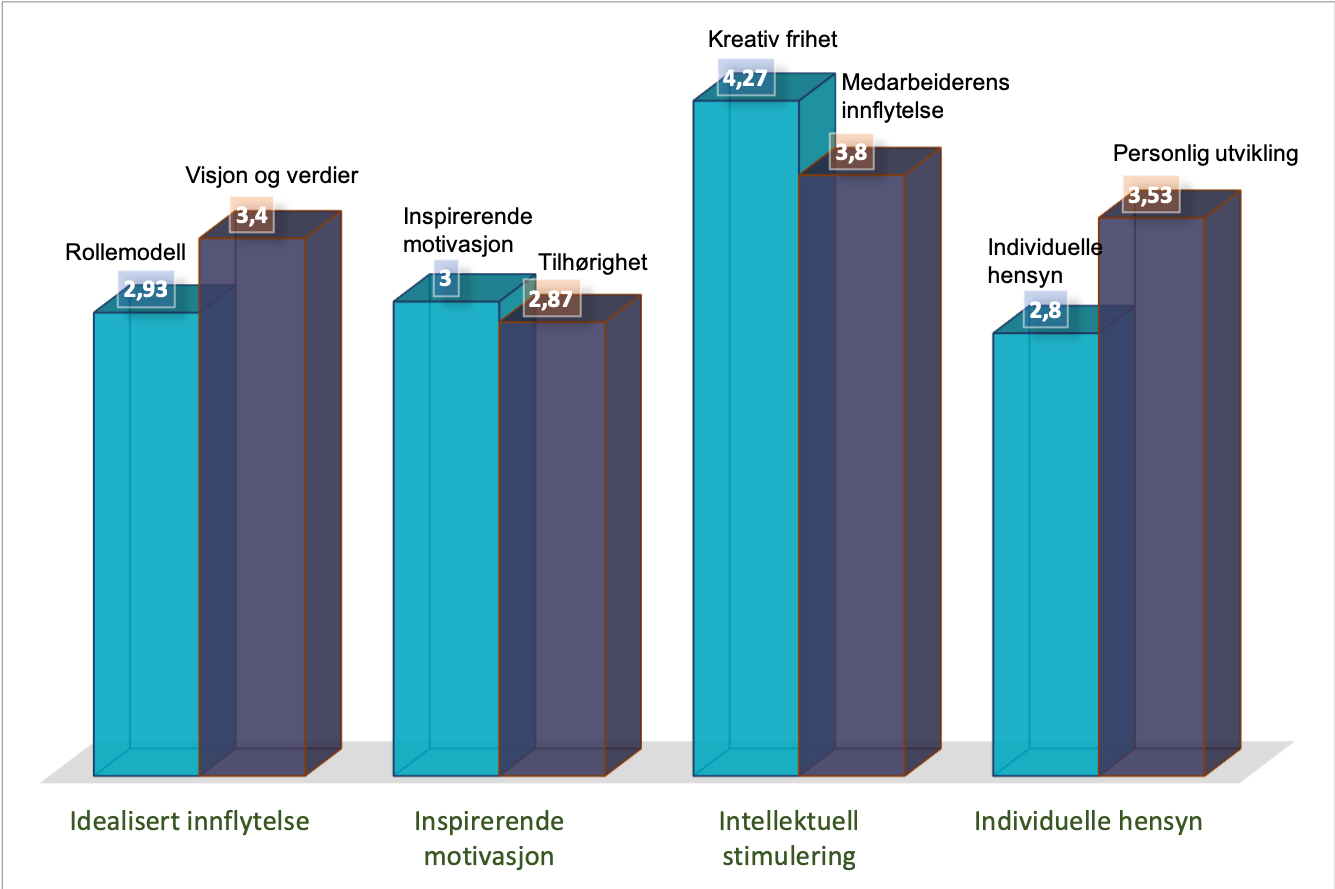
\includegraphics [scale=0.6]{bilder/resultat.png}
\caption{Spørreundersøkelse - resultat}
\label{fig:resultat}
\end{figure}

\begin{itemize}
\item\textit{Idealisert innflytelse} -  Lederens evne til å opptre som rollemodell og formidle visjoner og verdier gjennom egne handlinger.
\begin{itemize}
\item\textit{Rollemodell} - 2,93 av 5,00 hvorav 80\% enten var nøytrale (3), uenig (2) eller svært uenig (1).
\item\textit{Visjon og verdier} -  3,4 av 5,00 hvorav 53\% enten var nøytrale (3), uenig (2) eller svært uenig (1).
\end{itemize}
Dybdeintervjuet viste til at medarbeiderne oppfatter lederne som hardtarbeidende, men retter for lite oppmerksomhet mot medarbeiderne.

\item\textit{Inspirerende motivasjon} - Lederens evne til å inspirere og motivere ved å skape tilhørighet til felles mål og ambisjoner.
\begin{itemize}
\item\textit{Motivasjon} - 3,00 av 5,00 hvorav 73\% enten var nøytale (3), uenig (2) eller svært uenig (1).
\item\textit{Tilhørighet} - 2,87 av 5,00 hvorav 73\% enten var nøytale (3), uenig (2) eller svært uenig (1). 
\end{itemize}

\item\textit{Intellektuell stimulering} - Lederens evne til å fremme kreativitet og innovativ atferd.
\begin{itemize}
\item\textit{Individuelle hensyn} - 2,80 av 5,00 hvorav 87\% enten var nøytrale (3), uenig (2) eller svært uenig (1).
\item\textit{Personlig utvikling} - 3,53 av 5,00 hvorav 47\% enten var nøytrale (3), uenig (2) eller svært uenig (1). 
Årsaken til dette ble forklart av medarbeideren som en konsekvens av lite tilstedeværelse blant de ansatte, grunnet stress og fokus på kunder.
\end{itemize}

\item\textit{Individuelle hensyn} - Lederens evne til å samhandle og ta hensyn til individuelle behov for måloppnåelse og vekst.
\begin{itemize}
\item\textit{Kreativ frihet} - 4,27 av 5,00 hvorav 13\% enten var nøytrale (3), uenig (2) eller svært uenig (1). 
\item\textit{Inkludering ved viktige avgjørelser} - 3,80 av 5,00 hvorav 33\% var nøytale (3), uenig (2) eller svært uenig (1).
Intervjuobjektet (medarbeideren) beskrev de ansatte som tilfredse med ledernes evne til å oppfordre til kreativitet. I en del tilfeller blir imidlertid kreativitet begrenset grunnet budsjettrammer.
\end{itemize}
\end{itemize}

\indent \newline
På spørsmål knyttet til transaksjonsledelse fortalte Væhle at Involve ikke opererer med noe bonussystem i dag, og at dette heller ikke er vanlig for lignende bedrifter. 

\indent \newline
Avslutningsvis i begge intervjuene stilte vi spørsmål om det er andre utfordringer virksomheten burde ta tak i. Medarbeideren forklarte at de ansatte i perioder føler arbeidsmengden er for stor. Dette medfører at de blir tildelt prosjekter og arbeidsoppgaver som de ikke føler de behersker godt nok. Vi kontaktet Væhle ved en senere anledning for å forhøre oss om ledelsen er oppmerksomme på dette problemet. I følge hans oppfatning har ledelsen ikke blitt informert om dette, og er dermed ikke klar over medarbeidernes oppfatning angående arbeidsmengden. 

\indent \newline
Væhle fortalte i sitt intervju om utfordringer knyttet til samarbeid mellom avdelingene. Avdelingene blir holdt adskilt, i den forstand at hver enkelt avdeling har egne målsettinger og budsjetter å etterfølge. 
